\chapter{Durchführung}\label{chpt:durchfuerung}

Dieses Kapitel beschreibt die Durchführung des Projekts. Explizit wird hier der Beginn und Verlauf der Entwicklung der \glqq Leave The House\grqq-App behandelt. Zu Beginn wird der Start der Projektdurchführung, gefolgt von der eigentlichen Entwicklung beschrieben. Im Anschluss daran wird das Testen der Applikation behandelt. Zum Schluss dieses Kapitels werden in der Problembehandlung alle in den Anderen Abschnitten aufgetretenen Probleme ausführlich behandelt.

\section{Projektdurchführung}\label{sec:projektdurchfuerung}

Die Projektdurchführung behandelt den Start der eigentlichen Arbeit des Projekts. Wie bereits in \autoref{chpt:planung} beschrieben ist das Risiko des verspäteten Projektstarts eingetreten. Dies führte dazu, dass die Arbeit an dem Projekt nicht wie geplant am 01.01.2020 gestartet wurde. Der Projektstart begann stattdessen im März 2021. Durch die in der \nameref{sec:risiko} festgelegte Alternative hatte der verspätete Start keine, abgesehen der aus der Alternative resultierenden, Auswirkungen auf die Durchführung.\\
Die Bearbeitung des Projekts begann im März 2021 und endete mit Erreichung des geplanten Umfang Mitte April 2021. Durch die bereits genannte Erweiterung des Umfang nach Rücksprache mit dem Betreuer wird der endgültige Projektabschluss auf das Abgabedatum der Studienarbeit, den 17.05.2021, verlegt. Das Ende der Bearbeitung des zuvor geplanten Umfang wird weiterhin als Mitte April festgehalten. In der Verlängerten Bearbeitungszeit wird versucht die weiteren Ideen für den Umfang des Betreuer zu implementieren, da in dieser Zeit auch die Studienarbeit geschrieben werden muss kann eine vollständige Dokumentation dieser in der Studienarbeit nicht gewährleistet werden.

\section{Entwicklung}\label{sec:entwicklung}
In diesem Abschnitt wird der vollständige Verlauf der Entwicklung behandelt. Von der Erstellung des Projekts bis hin zum ersten fertigen Zustand der App. Die während der Entwicklung aufgetretenen Probleme werden hier genannt, jedoch erst im \autoref{sec:problem} \nameref{sec:problem} ausführlich behandelt. Das erstellen der im Umfang festgelegten Tests wird ebenfalls in einem anderen Abschnitt (\ref{sec:tests} \nameref{sec:tests}) behandelt.

\subsection{Projekterstellung}\label{subsec:projekterstellung}
Zu Beginn der Arbeit an einem Projekt muss zuerst das Projekt erstellt werden. Dies hängt damit zusammen, dass \acp{IDE} in der Regel Projekte als oberste Ordnerstruktur nutzen. Alle Dateien innerhalb des Projektordners können somit diesem Projekt zugeordnet werden.\\
Die Entwicklung der App begann ebenfalls mit der Erstellung eines neuen Projekts in Android Studio. Dabei wird \glqq New $\rightarrow$ New Project\grqq{} in der File Dropdown-Liste ausgewählt. Da Android nicht nur als Betriebssystem für Smartphones und Tablets sondern auch für Smartwatches oder in Autos und TVs verwendet wird muss als erster Schritt angegeben werden für welche Endplattform man eine Anwendung entwickeln möchte. In diesem Schritt kann auch direkt eine Projektvorlage ausgewählt werden. Aufgrund von geringer Erfahrung in der App-Entwicklung wurde für dieses Projekt die Vorlage \glqq Basic Activity\grqq (Basis Aktivität) anstatt einer \glqq Empty Activity\grqq (Leere Aktivität) als Grundlage für das Projekt gewählt. Im Gegensatz zu einer leeren Aktivität Vorlage beinhaltet die Basic Activity bereits ein Einstellungsmenü in der Werkzeugleiste am oberen Bildschirmrand, einem Knopf in der unteren Rechten Bildschirmecke und einen Knopf in der Mitte des Bildschirms, der einen Anzeigenwechsel bewirkt. Diese bereits vorhandenen Elemente und Funktionen erleichtern den Einstieg in die Entwicklung, da der Entwickler sich den Code dieser ansehen und somit leichter die Funktionsweise und Aufbau von Android-Apps verstehen kann. Hilfreich hierbei ist der in der Android Studio \ac{IDE} eingebaute Emulator. Mit dem Emulator können virtuelle Android Geräte erstellt werden, um die App zu testen. Dabei kann die Android Version, so wie das Gerät ausgewählt werden. Der Emulator ist direkt zu Projektstart der Punkt an dem das erste Problem auftrat. Nach erstellen des Projekts kann man die gewählte Vorlage direkt über den Emulator testen. Dafür muss im AVD Manager ein neues Gerät erstellt werden, welches zum testen genutzt werden soll. Bis hierhin lief alles reibungslos. Beim ausführen der App kam jedoch dann das Problem zum Vorschein, der Emulator konnte nicht gestartet werden.
Es blieben nun nur zwei Möglichkeiten das Problem zu beheben, welche im \autoref{sec:problem} \nameref{sec:problem} behandelt werden. Nach wählen der Vorlage müssen noch weitere Informationen bei der Projekterstellung angegeben werden.
Einerseits muss der Name des Projekts angegeben werden, hier wurde der Name der Endgültigen App \glqq Leave The House\grqq{} eingegeben. Andererseits müssen grundlegende Entscheidung für die Entwicklung der App gefällt werden. Neben dem Namen muss noch die Programmiersprache und die minimal kompatible Anrdoid-Version gewählt werden. Android Apps können in zwei verschiedenen Sprachen geschrieben werden. Java und Kotlin. Für dieses Projekt wurde Kotlin als Programmiersprache für die App ausgewählt. Kotlin ist in der Android Entwicklung weit verbreitet und bietet eine Interoperabilität für Java. Somit kann während der App-Entwicklung auch auf Java zurückgegriffen werden, falls dies nötig sein sollte. Kotlin bietet im Gegensatz zu Java weitere Features wie null-Absicherung zurm Schutz vor NullPointer-Exceptions oder direkte View.Bindung.\footcite{Kotlin.2020} Als minimale Android-Version wurde die \ac{API} (Programmierschnittstelle) 23 festgelegt. Diese entspricht der Android Version 6.0 Marshmello und wird laut Android Studio zum aktuellen Zeitpunkt von 84.9\% der Geräte unterstützt. Nach diesen Angaben wurde die Erstellung des Projekts in Android Studi erfolgreich abgeschlossen. An diesem Punkt (nach Behebung des Problems) könnte mit der Entwicklung begonnen werden, doch ein wichtiges weit verbreitetes und empfohlenes Mittel kann noch zum Projekt hinzugefügt werden. Die Versionsverwaltung.\\
Mithilfe von Versionsverwaltung können Änderungen an Dateien erfasst und verwaltet werden. Ein übliches Versionsverwaltungssystem ist der kostenlose Dienst GitHub. In GitHub können Nutzer für Projekte sogenannte \glqq Repository\grqq, zu Deutsch Verwaltungsorte, anlegen. Innerhalb eines Repository werden die Projektdateien verwaltet. GitHub erfasst jede Änderung an einer Datei und kann diese dem Nutzer anzeigen. Mithilfe eines commit können die Änderungen dann als neue Version im Repository abgelegt werden. Dies erlaubt es mehreren Nutzern an der gleichen Datei zu arbeiten ohne sich ständig in die Quere zu kommen. Außerdem erlaubt es dem Nutzer immer wieder auf stabile Versionen zurückzugreifen falls die aktuellen Änderungen nicht zum gewollten Ergebnis geführt haben. Im Zuge dieses Projektes wurde auf GitHub ein neues Repository angelegt, welches als Versionsverwaltung für die App genutzt wird. Damit können beispielsweise erfolgreiche Implementierungen eines Anwendungsfalls mithilfe eines commits in GitHub gesichert werden.\\
Mit der Erstellung des GitHub Repository und Verknüpfung des Android Studio Projekts damit ist die Projekterstellung abgeschlossen. Alle Vorbereitungen sind somit getroffen worden um eine Erfolgreiche Entwicklung zu gewährleisten.


\subsection{Erstellen der Checkliste}\label{subsec:erstelleChecklisten}

Nach der erfolgreichen Projekterstellung begann die Arbeit an dem Projekt mit der Realisierung des ersten Anwendungsfall, dem erstellen einer Checkliste. Dafür wurde die Klasse Checkliste angelegt, diese wird in \autoref{code:checkliste} gezeigt. Die Klasse besteht aus einem initialen Konstruktor, welcher den Titel und die Beschreibung, sowie einem zweiten Konstruktor der neben Titel und Beschreibung noch eine Liste von Aufgaben entgegennimmt. Zudem enthält die Klasse, wie in \autoref{sec:umfang} beschrieben, die Methoden um ein Element der Aufgaben Liste hinzuzufügen und um ein Element aus der Liste zu entfernen. Die ebenfalls beschrieben get() und set() Methoden sind in dieser Klasse nicht vorhanden, da Kotlin diese Methoden standardmäßig durch Zugriff auf die Variable zur Verfügung stellt. Um also auf den Titel einer Checkliste zuzugreifen genügt $checklist.title$ anstelle von $checklist.getTitle()$. Nachdem das Modell zum halten der Checkliste, die Checkliste-Klasse erstellt wurde muss nun die Funktion implementiert werden ein Checklisten Objekt zu erstellen und auf dem Bildschirm anzuzeigen.
\\
\lstinputlisting[
label=code:checkliste,    % Label; genutzt für Referenzen auf dieses Code-Beispiel
caption=Checkliste Klasse,
captionpos=b,               % Position, an der die Caption angezeigt wird t(op) oder b(ottom)
style=EigenerKotlinStyle,     % Eigener Style der vor dem Dokument festgelegt wurde
firstline=1,                % Zeilennummer im Dokument welche als erste angezeigt wird
lastline=14                 % Letzte Zeile welche ins LaTeX Dokument übernommen wird
]{Quellcode/Checkliste.kt}

Bevor diese Funktion jedoch implementiert werden kann muss der Ablauf dafür festgelegt werden. Der Nutzer soll auf den in der rechten unteren Bildschirmecke befindlichen Knopf drücken um eine neue Ansicht zu öffnen. Diese zeigt Eingabefelder für den Titel und die Beschreibung in denen der Benutzer diese Angaben tätigt, welche dann für den Konstruktor der Checklisten Klasse genutzt werden. Über einen Knopf an der gleichen Position wie der vorherige wird die Eingabe bestätigt und die Checkliste mit den Eingegeben Werten erstellt. Die erstellte Checkliste soll dann als Element einer Liste auf dem Bildschirm dargestellt werden. Anhand dieses Ablaufs wurde dann die Implementation dieser Funktion und Anwendungsfall begonnen. \autoref{fig:mainActivity} und \autoref{fig:createChecklist} zeigen die Layouts zu dem beschrieben Ablauf.\\
Android besteht Grundlegend aus Aktivitäten. Die Grundaktivität ist die sogenannte \glqq Main Activity\grqq. Diese bildet den Einstiegspunkt in die App und wird beim öffnen der App angezeigt. Eine Aktivität besteht meistens aus einer \grqq Controller-\grqq{} und einer Layout Datei. In der Layout-Datei wird definiert was auf dem Bildschirm angezeigt wird wenn die Aktivität ausgeführt wird. Dabei handelt es sich um eine XML-Datei in der Elemente wie Knöpfe, Text oder weitere mithilfe eines Layouts angeordnet werden können. Die Controller-Datei spiegelt dagegen die funktionale Ebene der Aktivität wieder. In ihr werden Funktionen ausgeführt und der Aktivitäts-Lebenszyklus behandelt. Eine Aktivität hat einen Lebenszyklus der aus verschiedenen Zuständen besteht. Der erste Zustand der ausgeführt wird ist \glqq onCreate()\grqq. In dieser Methode wird angegeben welches Layout dem Nutzer angezeigt werden soll. Diese Methode wird in der Regel immer überschrieben, um mittels setContentView() das Layout anzugeben. \autoref{code:onCreate} zeigt die onCreate-Methode der Aktivität CreateChecklist. Hier wird wie angegeben die onCreate-Methode überschrieben und über setContentView das zugehörige Layout zur Darstellung auf dem Bildschirm angegeben. Zudem wird über die seSupportActionBar-Methode die im Layout definierte Werkzeugleiste als SupportActionBar festgelegt. Damit wird der Aktivität ermöglicht die Interaktion mit eventuell in der Werkzeugleiste vorhanden Knöpfen zu erfassen und entsprechende Funktionen auszuführen. In der weiteren Beschreibung zur Implementierung des Anwendungsfall zum erstellen einer Aktivität wird weiter auf das Codebeispiel eingegangen. Die weiteren Zustände des Lebenszyklus sind onStart() (Startet die Aktivität und macht sie sichtbar und ermöglicht Interaktivität), onResume() (Wird ausgeführt wenn die Aktivität wieder Interagierbar wird), onPause() (Dieser Zustand tritt auf wenn die Aktiviät den Fokus verliert und ist oft ein Indikator dass die Aktivität verlassen wird), onStop() (Die Aktivität ist nicht länger sichtbar für den Nutzer), onRestart(Wechsel von onStop() in onStart()) und onDestroy() (Zerstört die Aktivität und endet den Lebenszyklus).\footcite{Aktivitäten.2021} Die Grundlegende Funktionsweise von Aktivitäten sollte nun verstanden worden sein.\\
Um den Anwendungsfall eine Checkliste erstellen zu realisieren wird zunächst eine neue Aktivität erstellt. Dazu wird über File $\rightarrow$ New $\rightarrow$ Activity $\rightarrow$ Empty Activity eine neue Aktivität angelegt. Hierbei muss der Name der Aktivität und des Layout angegeben werden. Der Name des Layout wird von Android Studio passend zu der Eingabe im Aktivitätsnamen-Feld angepasst. Auch hier kann die Programmiersprache gewählt werden. Das lässt sich auf die Interoperabilität zurückführen, da damit auch eine Java-Aktivität in einer Kotlin Anwendung ausgeführt werden kann.\\
In der onCreate-Methode wird wie bereits verdeutlicht das Layout für die Aktivität festgelegt. Das für die CreateActivity erstellte Layout kann in \autoref{fig:createChecklist} eingesehen werden. Es stellt jeweils ein Label sowie ein Eingabefeld für den Titel und die Beschreibung dar. Zusätzlich befindet sich in der unteren rechten Ecke ein Knopf über den die Checkliste mit den Eingaben aus den Eingabefeldern hinzugefügt werden soll.\\
Um dieses Layout auf dem Bildschirm zu sehen muss zunächst die dazugehörige Aktivität gestartet werden. Wie bereits erläutert wird die App mit der MainActivity gestartet, welche als Einstiegspunkt für die Anwendung dient. Das Layout der MainActivity kann in \autoref{fig:mainActivity} angesehen werden. Dieses Layout besteht aus einer Werkzeugleiste, der bereits im Ablauf für den Anwendungsfall beschriebene Liste in Form einer RecyclerView zum Anzeigen der Checklisten und dem aus der Vorlage übernommenen und angepassten Knopf. Mit diesem Knopf soll der Anwendungsfall und die createChecklist Aktivität gestartet werden. Um dem Knopf die Funktionalität dafür zu geben wird er zunächst über die findViewById-Methode der Knopf mithilfe der ID gefunden, um so mit ihm innerhalb dieser Klasse interagieren zu können. Für die Interaktion wird der Knopf mit einem onClickListener versehen. Dieser führt die darin geschriebene Funktion aus sobald der Nutzer den Knopf betätigt. In diesem Fall soll die CreateChecklist Aktivität gestartet werden. Dazu wird ein Intent deklariert. Ein Intent ist ein Nachrichten-Objekt das genutzt wird um Aktionen von einer anderen Anwendungskomponente anzufragen. Das starten einer Aktivität stellt einen der drei fundamentalen Anwendungsfälle des Intent Objekts dar.\footcite{Intents.2021} Der Codeausschnitt \autoref{code:onCreateInMain} zeigt die Deklaration des Intent un der darauffolgende Aufruf zum starten der CreateChecklist Aktivität im onClickListener des Knopf. Bei der Initialisierung des Intent muss die jeweilig zu startende Aktivität als Parameter übergeben werden. Diese wird im Anschluss mit dem Befehl startActivity() oder in diesem Fall startActivityForResult() durch Übergabe des Intent in den Befehl gestartet. Zusätzlich wird beim Starten der Aktivität ein weiterer Parameter übergeben. Dieser stellt einen requestCode dar mit dessen Hilfe Ergebnisse von Aktivitäten unterschieden werden können. Das ermöglicht den korrekten Umgang mit den im Ergebnis potentiell übergebenen Daten.
\\
\lstinputlisting[
label=code:onCreateInMain,    % Label; genutzt für Referenzen auf dieses Code-Beispiel
caption=Start der CreateChecklist Aktivität,
captionpos=b,               % Position, an der die Caption angezeigt wird t(op) oder b(ottom)
style=EigenerKotlinStyle,     % Eigener Style der vor dem Dokument festgelegt wurde
firstline=1,                % Zeilennummer im Dokument welche als erste angezeigt wird
lastline=4                 % Letzte Zeile welche ins LaTeX Dokument übernommen wird
]{Quellcode/startOnCreateInMain.kt}

Nachdem die Aktivität gestartet wurde wird, wie mit dem Aktivitäts-Lebenszyklus beschreiben die onCreate-Methode der CreateChecklist Aktivität ausgeführt. Wie in \autoref{code:onCreate} zu sehen wird dort ebenfalls der Knopf mit einem onClickListener versehen. Dieser beendet im Gegensatz zum anderen die Aktivität anstatt eine neue MainActivity zu starten. Allerdings wird ebenfalls ein Intent erstellt. Mithilfe des Intent werden die Nutzereingaben der MainActivity als Ergebnis der createActivity Aktivität übergeben. Um die Nutzereingaben zu lesen werden die Textfelder, wie die Knöpfe zuvor, mithilfe der ID gefunden un der deren Text-Attribut ausgelesen. Die putExtra-Methode des Intent erlaubt es über einen Intent zusätzliche Daten zu übergeben. Dazu muss in dieser Methode ein Schlüssel-Wert Paar erstellt werden. Nachdem die Nutzereingaben dem Intent beigefügt wurden wird dieser in der setResult-Methode zusammen mit einem RequestCode übergeben. Der RequestCode spiegelt hier den gleichen wieder der auch zum starten der Aktivität übergeben wurde. Die zwei darauffolgenden Methodenaufrufe dienen dem Beenden der Aktivität.
Das Ergebnis wird durch die onActivityResult-Methode weiter verarbeitet, welche in \autoref{code:onActivityResult} teilweise einsehbar ist. Diese wird, wie die onCreate-Methode, überschrieben um eigenen Code ausführen zu können. Die Methode bekommt als Parameter einen RequestCode, einen resultCode und einen Intent als Datenhalter übergeben. Hier wird der Nutzen des requestCode deutlich. Er wird als Schlüsselvariable für den Switch genutzt, um Ergebnisse aus unterschiedlichen Aktivitäten unterscheiden zu können. Für den Aktuellen Stand von nur einer Aktivität wäre der Switch nicht notwendig, da im weiteren verlauf der Entwicklung weitere hinzukommen wurde er bereits von Anfang an implementiert. Der resultCode stellt den Status des Ergebnis der Aktivität dar und könnte beispielsweise Result.OK lauten. Dieser findet hier allerdings keine Verwendung da die Ergebnisüberprüfung über ein Extra des Intent behandelt wird. Bei dem Intent handelt es sich um den in der setResult-Methode übergebenen Intent. Zu Beginn der Bearbeitung der vom Intent übergebenen Daten wird über das \glqq successful\grqq{}-Extra geprüft ob das übergeben der Daten erfolgreich war. Im Anschluss wird ein neues Checklisten-Objekt erstellt. Dieses erhält als Parameter die vom Nutzer in der CreateChecklist Aktivität eingegebenen Titel und Beschreibung. Im Anschluss daran wird überprüft ob der Eingegebene Titel ein Duplikat ist. Falls dem so ist wird die neue Checkliste nicht der Liste von Checklisten zugefügt, welche als Datenhalter in der Main-Aktivität dient, und eine Fehlermeldung auf dem Bildschirm angezeigt. Falls nicht wird die neue Checkliste der Liste hinzugefügt und infolgedessen auf dem Bildschirm angezeigt.
\\
\lstinputlisting[
label=code:onCreate,    % Label; genutzt für Referenzen auf dieses Code-Beispiel
caption=onCreate Methode der CreateChecklist Aktivität,
captionpos=b,               % Position, an der die Caption angezeigt wird t(op) oder b(ottom)
style=EigenerKotlinStyle,     % Eigener Style der vor dem Dokument festgelegt wurde
firstline=1,                % Zeilennummer im Dokument welche als erste angezeigt wird
lastline=21                 % Letzte Zeile welche ins LaTeX Dokument übernommen wird
]{Quellcode/onCreate.kt}

\lstinputlisting[
label=code:onActivityResult,    % Label; genutzt für Referenzen auf dieses Code-Beispiel
caption=onActivityResult Methode der Main Aktivität,
captionpos=b,               % Position, an der die Caption angezeigt wird t(op) oder b(ottom)
style=EigenerKotlinStyle,     % Eigener Style der vor dem Dokument festgelegt wurde
firstline=1,                % Zeilennummer im Dokument welche als erste angezeigt wird
lastline=25                 % Letzte Zeile welche ins LaTeX Dokument übernommen wird
]{Quellcode/onActivityResult.kt}

Die Checklisten sollen in Form einer Liste auf dem Bildschirm dargestellt werden. Dazu wird wie im Layout der MainActivity beschrieben eine RecyclerView genutzt. Im Vergleich zu einer herkömmlichen ListView ist die RecyclerView eine modernere, flexiblere und performantere Alternative. Im Gegensatz zu Knöpfen und Textfeldern kann die RecyclerView nicht einfach mithilfe der ID gefunden und beispielsweise der Text gesetzt werden. Um Einträge in der RecyclerView anzuzeigen wird ein Adapter benötigt. Das ist Notwendig da jedes Item in der Liste als separate View behandelt wird und gesondert dargestellt werden muss. Um die Checklisten in der RecyclerView darstellen zu können wurde der ChecklistRecyclerViewAdapter als Klasse angelegt. Dieser erhält als Parameter die Liste von Checklisten aus der MainActivity, da diese die Informationen zu den Items hält die Dargestellt werden sollen. Zusätzlich wird innerhalb dieser Klasse eine weitere Klasse erstellt. Diese Klasse ist ein ViewHolder und heißt ChecklistViewHolder. Jedes Item in der RecyclerView wird durch eine Instanz dieses ViewHolder definiert. Für jeden Eintrag in der Liste wird vom Adapter ein ViewHolder erstellt und im Anschluss daran die Daten daran gebunden. \autoref{code:ViewHolder} zeigt die Methoden onCreateViewHolder und onBindViewHolder des ViewHolder. Ähnlich wie bei den Aktivitäten wird in der onCreate-Methode das Layout festgelegt. Bei dem Layout handelt es sich um ein speziell für die Liste erstelltes Layout, welches einen Eintrag der Liste repräsentiert. In \autoref{fig:mainActivity} können drei dieser Listenitems gesehen werden. Diese bestehen aus einem Textfeld für den Titel der Checkliste und einem weiteren, etwas nach rechts gerücktem, mit kleinerer und grauer Textfont versehenen Textfeld für die Beschreibung. Die onBindViewHolder-Methode setzt den Text dieser Textfelder, sodass die richtigen Daten angezeigt werden.
In der MainActivity wird um die Daten darzustellen die RecyclerView anhand der ID gefunden und eine Instanz des Adapter erstellt. Dabei wird die Liste der Checkliste als darzustellende Items übergeben. Damit frisch erstellte Checklisten in der Liste angezeigt werden wurde die onActivityResult-Methode um dem Funktionsaufruf 
$checklistRecyclerView.adapter?.notifyDataSetChanged()$ erweitert. Dieser teilt dem Adapter mit, dass sich die Daten verändert haben und veranlasst so ein neu laden der Liste.\\
\\
\lstinputlisting[
label=code:ViewHolder,    % Label; genutzt für Referenzen auf dieses Code-Beispiel
caption=ViewHolder Methoden des ChecklistRecyclerViewAdapter,
captionpos=b,               % Position, an der die Caption angezeigt wird t(op) oder b(ottom)
style=EigenerKotlinStyle,     % Eigener Style der vor dem Dokument festgelegt wurde
firstline=1,                % Zeilennummer im Dokument welche als erste angezeigt wird
lastline=12                 % Letzte Zeile welche ins LaTeX Dokument übernommen wird
]{Quellcode/ViewHolder.kt}

\begin{figure}[h]
	\centering
	\begin{minipage}{0.45\linewidth}
		\centering
		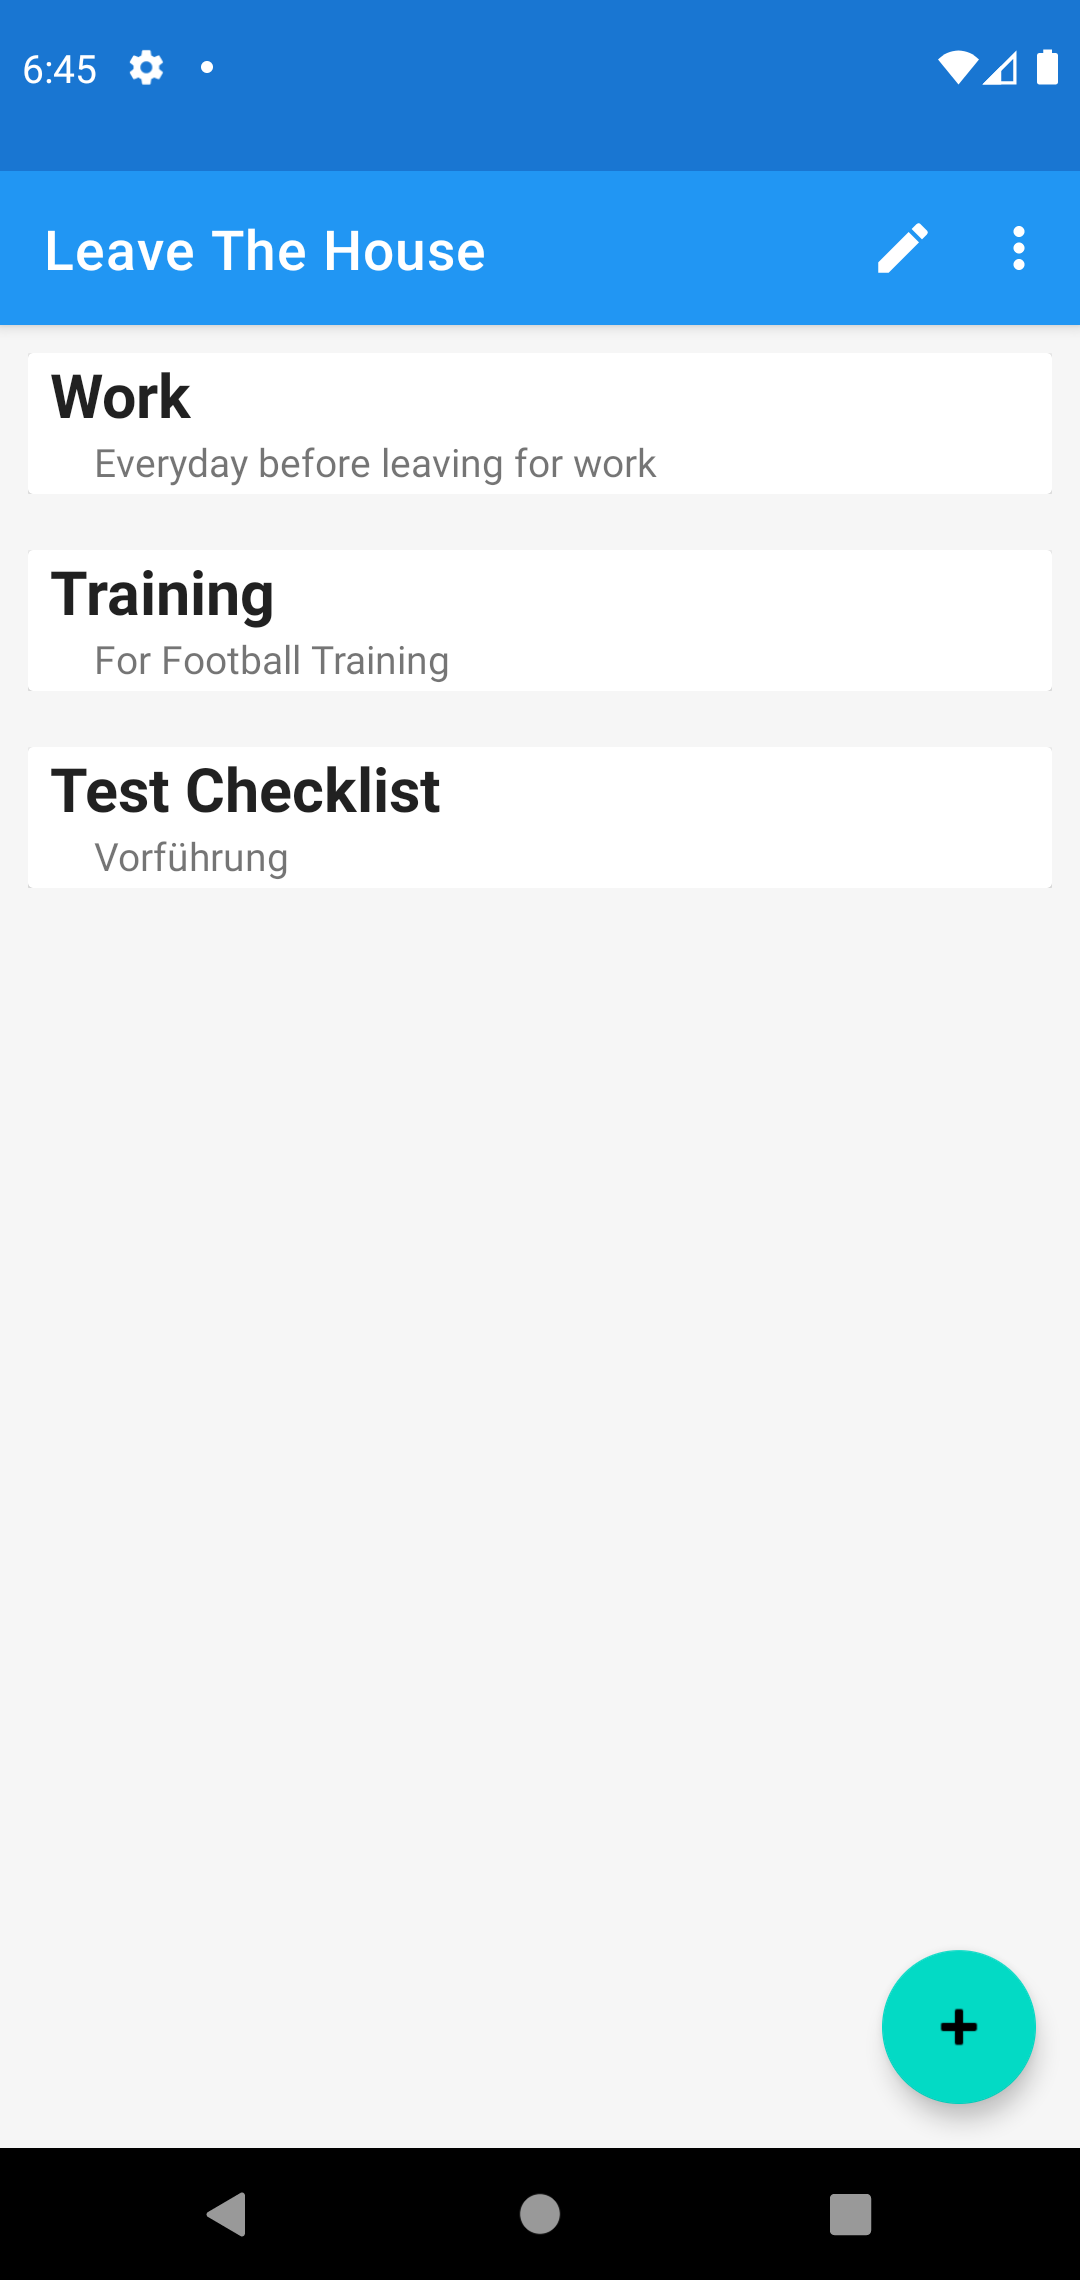
\includegraphics[width=.9\linewidth]{Bilder/MainActivity.png}
		\caption{MainActivity Ansicht}
		\label{fig:mainActivity}
	\end{minipage}
	\hfill
	\begin{minipage}{0.45\linewidth}
		\centering
		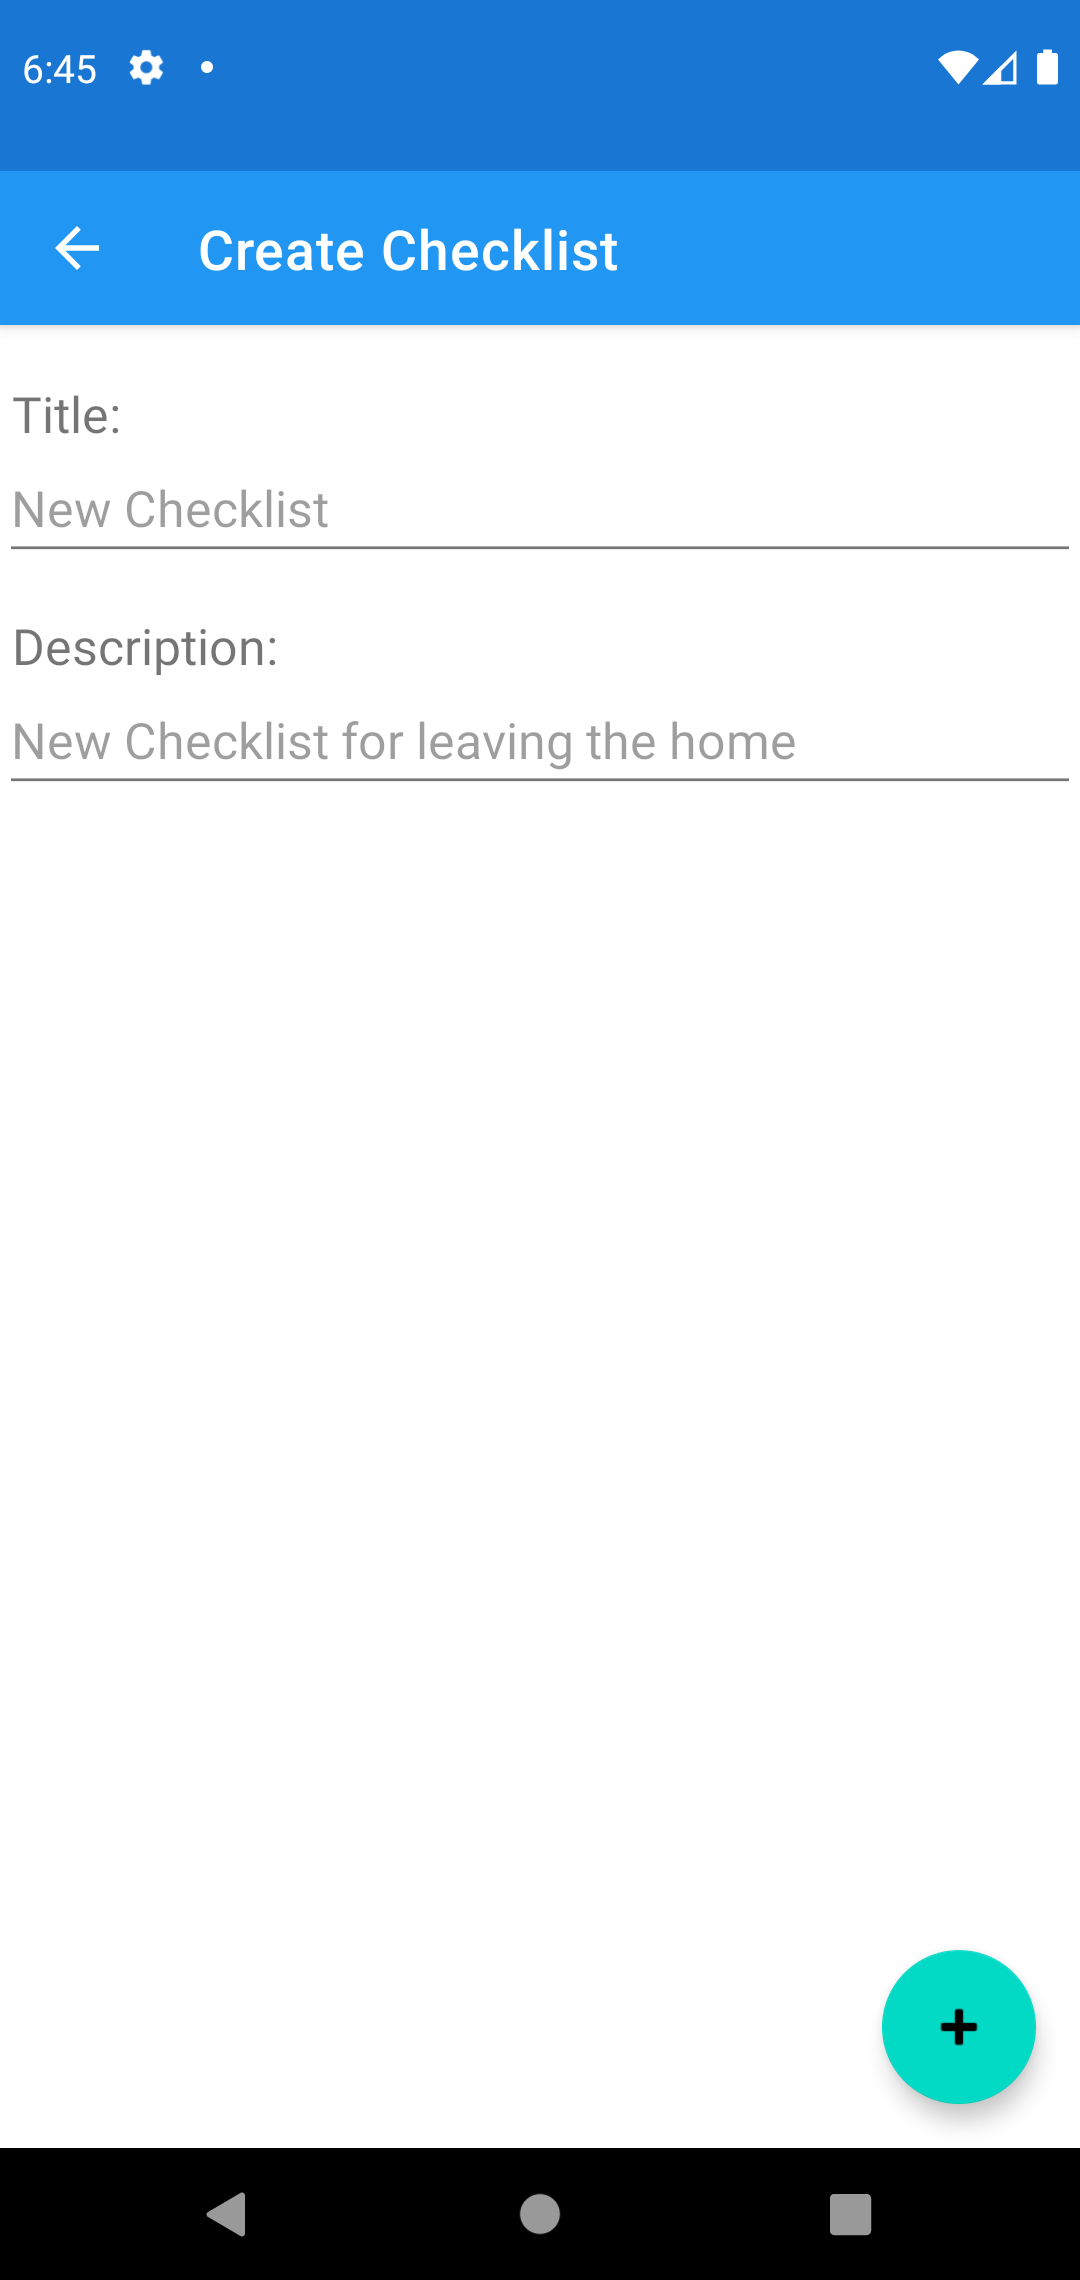
\includegraphics[width=.9\linewidth]{Bilder/CreateChecklist.png}
		\caption{CreateChecklist Ansicht}
		\label{fig:createChecklist}
	\end{minipage}
\end{figure}

Mit dem darstellen der erstellten Checkliste kann der erste Anwendungsfall, das erstellen einer Checkliste, als erfolgreich implementiert angesehen werden. Es ist dem Nutzer möglich über den Knopf die CreateChecklist Aktivität zu starten und seine Eingaben für Titel und Beschreibung zu tätigen. Durch bestätigen der Eingaben wird das neue Checklisten Objekt erstellt und dynamisch in der RecyclerView-Liste eingefügt und dargestellt.

\subsection{Speichern von Checklisten}\label{subsec:speichereCheckliste}

\subsection{Erstellen von Aufgaben}\label{subsec:erstelleAufgaben}

\subsection{Erweiterung}\label{subsec:erweiterung}

\section{Tests}\label{sec:tests}

\section{Problembehandlung}\label{sec:problem}